% Drawing 74/02-6 -- folder 74, batch 02, archive page 28 (PDF page 29).
% Transcription: un triangle épais d'où rayonnent de nombreux triangles plus fins, en éventail, suivi d'une accolade.
% Kind: fan of triangles around a thick triangle. Method 2 (schematic redraw from the facsimile). Status: partial.
% Notes: A thick triangle with many thin triangles radiating from it; the thin ones are drawn as representative strokes (their number is not countable on the page). The brace that follows lies just right of the bbox and is not drawn.
% Coordinates: 1 unit = 1 mm = 1/100 of the crop width (bbox in page fractions: [0.3, 0.45, 0.5, 0.56]).
% Redrawn by Claude (claude-opus-5-5), issue #73, 2026-11-07; not checked by a human; not compiled (no TeX in the session).
% Rights: reproduces part of the work -- behind RENDER_TRANSCRIPTS, never published by itself.
\documentclass[tikz,border=3pt]{standalone}
\usepackage{amsmath,amssymb}
\usetikzlibrary{patterns,arrows.meta}
\tikzset{pencil/.style={black!45}, struck/.style={black!35}, mark/.style={circle,draw,inner sep=1.3pt}, pt/.style={circle,fill,inner sep=0.9pt}, opt/.style={circle,draw,fill=white,inner sep=1.1pt}}
\begin{document}
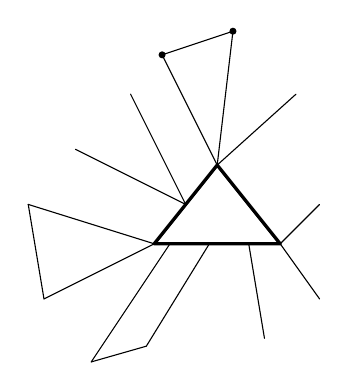
\begin{tikzpicture}[x=1mm,y=1mm,line cap=round,line join=round,font=\scriptsize]
\draw[very thick] (78,-45) -- (86,-35) -- (94,-45) -- cycle;
\draw (78,-45) -- (62,-40);
\draw (78,-45) -- (64,-52);
\draw (80,-45) -- (70,-60);
\draw (85,-45) -- (77,-58);
\draw (90,-45) -- (92,-57);
\draw (94,-45) -- (99,-52);
\draw (94,-45) -- (99,-40);
\draw (86,-35) -- (79,-21);
\draw (86,-35) -- (88,-18);
\draw (86,-35) -- (96,-26);
\draw (82,-40) -- (68,-33);
\draw (82,-40) -- (75,-26);
\draw (62,-40) -- (64,-52);
\draw (70,-60) -- (77,-58);
\draw (79,-21) -- (88,-18);
\node[pt] at (79,-21) {};
\node[pt] at (88,-18) {};
\end{tikzpicture}
\end{document}
